\documentclass[aspectratio=169]{beamer}\usepackage[]{graphicx}\usepackage[]{color}
% maxwidth is the original width if it is less than linewidth
% otherwise use linewidth (to make sure the graphics do not exceed the margin)
\makeatletter
\def\maxwidth{ %
  \ifdim\Gin@nat@width>\linewidth
    \linewidth
  \else
    \Gin@nat@width
  \fi
}
\makeatother

\definecolor{fgcolor}{rgb}{0.345, 0.345, 0.345}
\newcommand{\hlnum}[1]{\textcolor[rgb]{0.686,0.059,0.569}{#1}}%
\newcommand{\hlstr}[1]{\textcolor[rgb]{0.192,0.494,0.8}{#1}}%
\newcommand{\hlcom}[1]{\textcolor[rgb]{0.678,0.584,0.686}{\textit{#1}}}%
\newcommand{\hlopt}[1]{\textcolor[rgb]{0,0,0}{#1}}%
\newcommand{\hlstd}[1]{\textcolor[rgb]{0.345,0.345,0.345}{#1}}%
\newcommand{\hlkwa}[1]{\textcolor[rgb]{0.161,0.373,0.58}{\textbf{#1}}}%
\newcommand{\hlkwb}[1]{\textcolor[rgb]{0.69,0.353,0.396}{#1}}%
\newcommand{\hlkwc}[1]{\textcolor[rgb]{0.333,0.667,0.333}{#1}}%
\newcommand{\hlkwd}[1]{\textcolor[rgb]{0.737,0.353,0.396}{\textbf{#1}}}%
\let\hlipl\hlkwb

\usepackage{framed}
\makeatletter
\newenvironment{kframe}{%
 \def\at@end@of@kframe{}%
 \ifinner\ifhmode%
  \def\at@end@of@kframe{\end{minipage}}%
  \begin{minipage}{\columnwidth}%
 \fi\fi%
 \def\FrameCommand##1{\hskip\@totalleftmargin \hskip-\fboxsep
 \colorbox{shadecolor}{##1}\hskip-\fboxsep
     % There is no \\@totalrightmargin, so:
     \hskip-\linewidth \hskip-\@totalleftmargin \hskip\columnwidth}%
 \MakeFramed {\advance\hsize-\width
   \@totalleftmargin\z@ \linewidth\hsize
   \@setminipage}}%
 {\par\unskip\endMakeFramed%
 \at@end@of@kframe}
\makeatother

\definecolor{shadecolor}{rgb}{.97, .97, .97}
\definecolor{messagecolor}{rgb}{0, 0, 0}
\definecolor{warningcolor}{rgb}{1, 0, 1}
\definecolor{errorcolor}{rgb}{1, 0, 0}
\newenvironment{knitrout}{}{} % an empty environment to be redefined in TeX

\usepackage{alltt}
\usepackage{multirow}
%\usecolortheme{beaver}
%\usecolortheme[RGB={129,3,3}]{structure}
\usetheme{CambridgeUS}
\usecolortheme{seahorse}

% Standard header (will need to change date!)
\title[GEOG 5680 Summer '21]{GEOG 5680\\Introduction to R}
\subtitle[Intro]{00: Class Introduction}
\author[S. Brewer]{Simon Brewer}
\institute[Univ. Utah]{
  Geography Department\\
  University of Utah\\
  Salt Lake City, Utah 84112\\[1ex]
  \texttt{simon.brewer@geog.utah.edu}
}
\date[May 11, 2021]{May 11, 2021}
\IfFileExists{upquote.sty}{\usepackage{upquote}}{}
\begin{document}
%\SweaveOpts{concordance=TRUE}

%--- the titlepage frame -------------------------%
\begin{frame}
  \titlepage
\end{frame}

%--- Slide 1 ----------------%
% \begin{frame}{Outline}
% 
% \begin{itemize}
%   \item Introduction to course
% 	\begin{itemize}
% 		\item Course goals
% 	\end{itemize}
%     	\item Syllabus
% 	\begin{itemize}
% 	  \item Exercises
% 		\item Project
% 	\end{itemize}
% 	\item What is R?
% \end{itemize}
% \end{frame}
% 
% %--- Slide 2 ----------------%
% \begin{frame}{Contact Information}
% \begin{itemize}
% 	\item Email: simon.brewer@geog.utah.edu
% 	\item Office: Bldg 73 Room 204
%   \item Office hours: \emph{this week}
% \end{itemize}
% \end{frame}
% 
\section{Course Introduction}
%--- Slide 3 ----------------%
\begin{frame}{Course Goals}
\begin{itemize}
  \item This course is designed to give an intensive introduction to R for analysis, programming and as a graphical tool. The aims are to:
  \begin{itemize}
    \item Introduce R as a data analysis and statistical software tool
    \item Learn about manipulating data in R
    \item Use scripts and functions to help analyzing data
    \item Cover basic to more advanced plotting
    \item Look at the add-on packages that extend R's functions
    \item Introduce basic statistical modeling in R
  \end{itemize}
  \item<2-> It is aimed at people with little to no prior experience with R or programming, although some basic knowledge of statistics is assumed
  \item<3-> Designed as a series of modules: short video intro + computer exercises
\end{itemize}
\end{frame}

%--- Slide ----------------%
\begin{frame}{Syllabus}
\begin{itemize}
  \item 00: Class introduction
  \item 01: Data import and export
  \item 02: Data manipulation I
  \item 03: Basic plotting
  \item 04: Control functions and loops
  \item 05: R functions
  \item 06: Writing reports in R
  \item 07: Data manipulation II
\end{itemize}
\end{frame}

%--- Slide ----------------%
\begin{frame}{Syllabus}
\begin{itemize}
  \item 08: Extending basic plots with \textbf{ggplot2}
  \item 09: Simple inference tests
  \item 10: Introduction to statistical modeling in R
  \item 11: Data manipulation III
  \item 12: Making maps in R
  \item 13: Using Github with R
  \item 14: Web applications with Shiny
  \item 15: Optional modules (mixed-effects models, interactive maps, ...)
\end{itemize}
\end{frame}

%--- Slide 15 ----------------%
\begin{frame}{Reading material}
\begin{columns}
  \begin{column}{0.5\textwidth}
    Dalgaard, Introductory statistics with R (Springer)
  	\begin{center}
			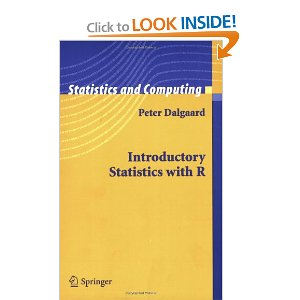
\includegraphics[width=0.7\textwidth]{./images/dalgaardbook.jpg}
		\end{center}
	\end{column}
	\begin{column}{0.5\textwidth}
    Grolemund, Hands-on Programming with R (O'Reilly)
		\begin{center}
			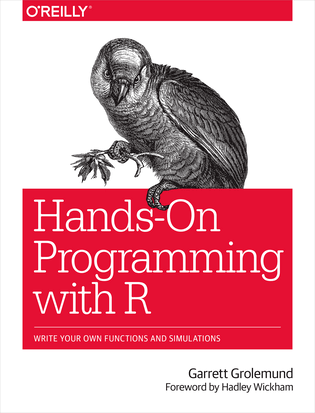
\includegraphics[width=0.6\textwidth]{./images/handsonR.png}
		\end{center}
	\end{column}
\end{columns}
\end{frame}

%--- Slide 14 ----------------%
% \begin{frame}{Reading Material}
% Other material
% \begin{itemize}
% 	\item Kuhnert, P. and W. Venables, 2005, An Introduction to R:  Software for Statistical Modelling \& Computing.  CSIRO Australia (PDF)
% 	\item Owen, W.J., 2007, The R Guide.  Dept. of Mathematics and Computer Science, University of Richmond.  (PDF)
% 	\item Bivand, R.S., E.J. Pebesma, and V. Gomez-Rubio (2008).  Applied Spatial Data Analysis with R.  Springer, 374 pp. (PDF)
% \end{itemize}
% \end{frame}

%--- Slide 9 ----------------%
\begin{frame}{Course assessment}
\begin{itemize}
  \item In-class exercises (45 pts)
  \begin{itemize}
    \item 2-3 short exercises per class
    \item Designed to make you repeat the methods covered
    \item Provide R code as a script
    \item Copy-paste results and/or figures to Word document
    \item Submission through Canvas
    \item All exercises to be submitted by Wednesday, June 17
  \end{itemize}
  \item<2-> Course project (55 pts)
  \begin{itemize}
    \item Analysis of a dataset using one or more of the techniques covered in class (or use R to explore other techniques)
    \item Project can be either:
  	\begin{itemize}
  		\item One of three predefined datasets
  		\item Your own dataset
  	\end{itemize}
  \end{itemize}
\end{itemize}
\end{frame}

%--- Slide 12 ----------------%
\begin{frame}{Course Project}
\begin{itemize}
  \item Examples of projects
  \begin{itemize}
  	\item Investigating the link between house characteristics and price
  	\item Factors influencing companies profits
  	\item Results of cloud seeding experiment
  \end{itemize}
  \item Project report - worth 55\% of overall grade
  \begin{itemize}
  	\item Projects to be written in R Markdown (covered in module 06)
  	\item Include:
  	\begin{itemize}
  		\item R Code
      \item Results including figures
      \item Brief discussion of project and results
  	\end{itemize}
  	\item Due Wednesday, June 17 through Canvas
  \end{itemize}
\end{itemize}
\end{frame}

\section{Introduction to R}
%--- Slide 15 ----------------%
\begin{frame}{Introduction to R}
\begin{columns}
	\begin{column}{0.35\textwidth}
		\begin{itemize}
			\item GNU GPL (free) statistical language and environment
			\item Comprehensive R Archive Network (CRAN)
			\item www.r-project.org
		\end{itemize}
	\end{column}
	\begin{column}{0.65\textwidth}
		\begin{center}
			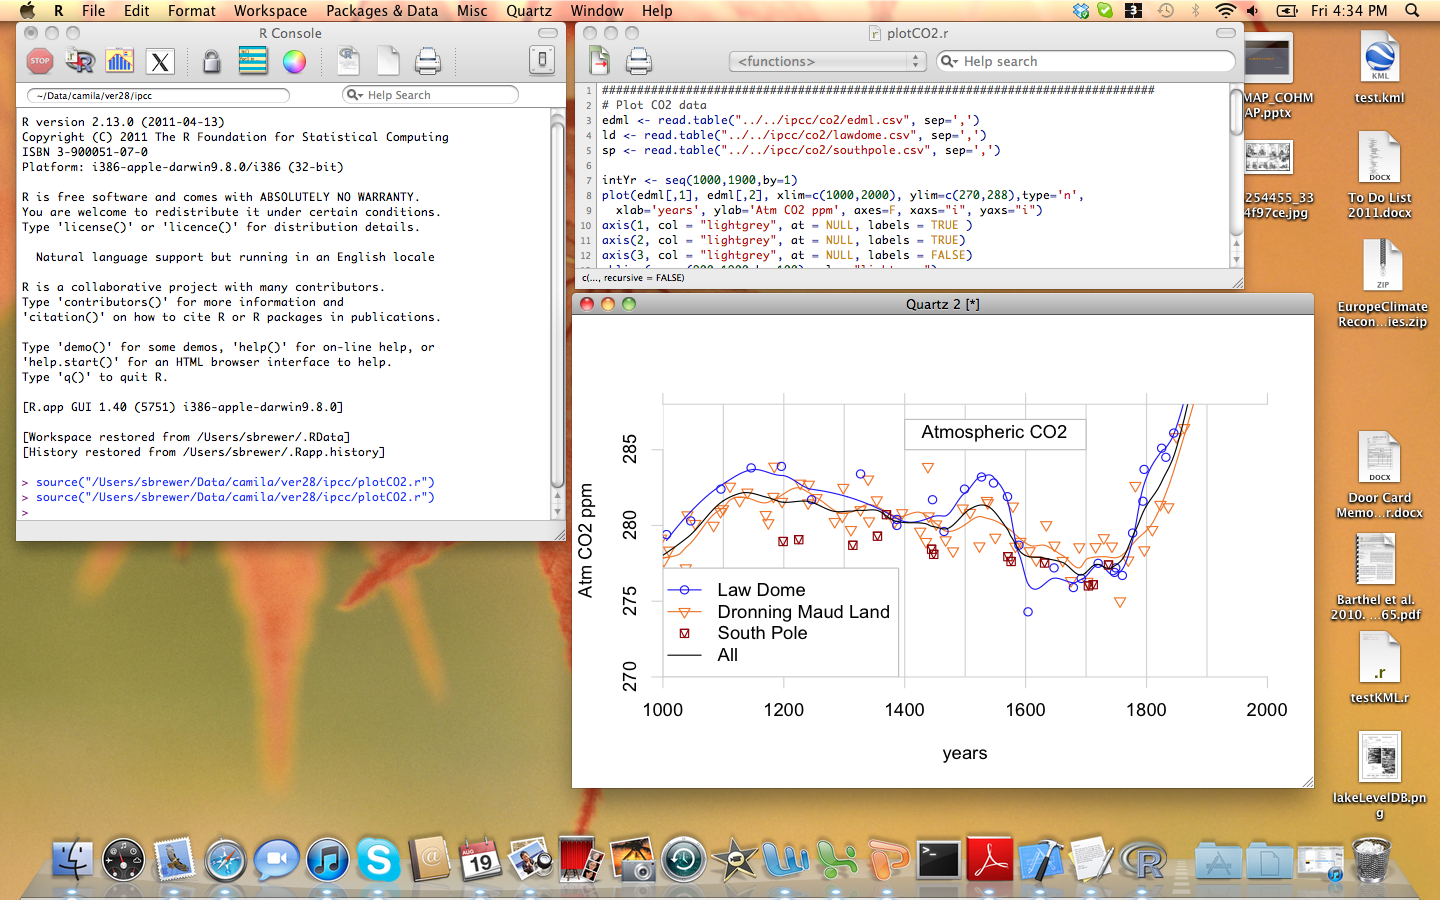
\includegraphics[width=1.0\textwidth]{./images/R_screen.png}
		\end{center}
	\end{column}
\end{columns}
\end{frame}

%--- Slide 16 ----------------%
\begin{frame}{What is R?}
R is an integrated suite of software facilities for data manipulation, calculation and graphical display. Among other things it has
\begin{itemize}
	\item an effective data handling and storage facility,
	\item a suite of operators for calculations on arrays, in particular matrices,
	\item a large, coherent, integrated collection of intermediate tools for data analysis,
	\item graphical facilities for data analysis and display either directly at the computer or on hardcopy, and
	\item a well developed, simple and effective programming language (called `S') which includes conditionals, loops, user defined recursive functions and input and output facilities. 
\end{itemize}
\end{frame}

%--- Slide 17 ----------------%
\begin{frame}{What is R?}
%Why R?
\begin{itemize}
	\item Programming language + interfaces
	\item Extensive graphics capability
	\item Easily transferable --- runs on Mac/Windows/Unix
	\item Free, open source!
	\item Highly extensible
	\begin{itemize}
		\item Large number of existing functions/packages
		\item Ability to write personal functions
	\end{itemize}
	\item Capability for mapping data, an asset not generally available in other statistical software
	\begin{itemize}
  	\item Several add-on packages specifically designed for the analysis of time and space data
	\end{itemize}
	\item Increasingly used in many disciplines
\end{itemize}
\end{frame}

%--- Slide 15 ----------------%
\begin{frame}{Why learn R?}
\begin{columns}
  \begin{column}{0.5\textwidth}
    \begin{itemize}
      \item ``Programming tools: Adventures with R''
      \item Tippman, Nature Dec. 2014
    \end{itemize}
	\end{column}
	\begin{column}{0.5\textwidth}
		\begin{center}
			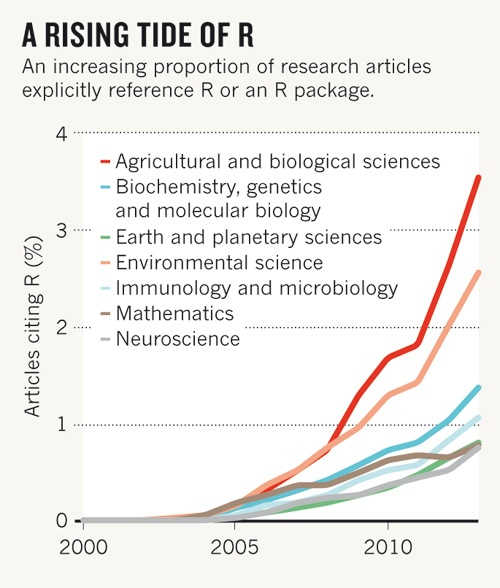
\includegraphics[width=0.8\textwidth]{./images/nature.jpg}
		\end{center}
	\end{column}
\end{columns}
\end{frame}

%--- Slide ----------------%
\begin{frame}{Why learn R?}
\begin{itemize}
  \item R is the 21st highest paid tech skill (Dice Tech Salary Survey, 2016)
  \item R second most used data science language after Python (Kaggle, 2016)
  \item R is \#5 on list of most popular analytics jobs  (Indeed.com, Feb. 2017)
  \item R is ranked second in usage in data science articles (Google scholar, Feb. 2017)
  \item R growing faster than any other data science language used in research (Google scholar, Feb. 2017)
  \item R is \#5 on IEEE spectrum ranking (2019: search ranking, trends, social media, job postings)
  %\item R is the \#1 Google Search for Advanced Analytics software (Google Trends, March 2014)
\end{itemize}
\end{frame}

%--- Slide 15 ----------------%
\begin{frame}{Why learn R?}
		\begin{center}
			
\includegraphics[width=1.0\textwidth]{./images/RvsPython}
		\end{center}

From www.datacamp.com
\begin{columns}
  \begin{column}{0.5\textwidth}
    \begin{itemize}
      \item R focuses on better, user friendly data analysis, statistics and graphical models
      \item Used by statisticians who need to do some programming
    \end{itemize}
	\end{column}
	\begin{column}{0.5\textwidth}
    \begin{itemize}
      \item Python emphasizes productivity and code readability
      \item Used by programmers who need to do some statistics
    \end{itemize}
	\end{column}
\end{columns}
\end{frame}

% %--- Slide 18 ----------------%
% \begin{frame}{Why learn R?}
% \begin{itemize}
%   \item Capability for mapping data, an asset not generally available in other statistical software
% 	\item Several add-on packages specifically designed for the analysis of time and space data
%   \item Used in data mining and bioinformatics
% 	\item Reads most output from image processing, remote sensing and GIS software
% 	\item Interfaces directly to most databases: ODBC, SQL, ArcInfo, GRASS
% 	\item Interaces to popular APIs: e.g. Google vizualization, Apache Hadoop
% 	\item Increasing ability to work with big datasets (AWS, parallel processing)
% \end{itemize}
% \end{frame}
% 
%--- Slide 19 ----------------%
\begin{frame}{Why learn R?}
\textbf{But:}
\begin{itemize}
  \item No (or limited) graphical interface
	\item Data manipulation can be complex
	\item Limited documentation
	\item Steep learning curve
\end{itemize}
\end{frame}

\section{Brief introduction to R/RStudio}
%--- Slide 19 ----------------%
\begin{frame}{RStudio}
\begin{columns}
	\begin{column}{0.70\textwidth}
  Free integrated development enviroment (IDE) for R
  \begin{itemize}
    \item Better help functions
    \item Integrated script editor
  	\item More useful package manager
  	\item Access to current datasets
  	\item Plot history
  \end{itemize}
	\end{column}
	\begin{column}{0.3\textwidth}
		\begin{center}
			
\includegraphics[width=0.8\textwidth]{./images/rstudio_icon.png}
		\end{center}
	\end{column}
\end{columns}
\end{frame}

% %--- Slide 19 ----------------%
% \begin{frame}{RStudio}
%   	\begin{center}
% 			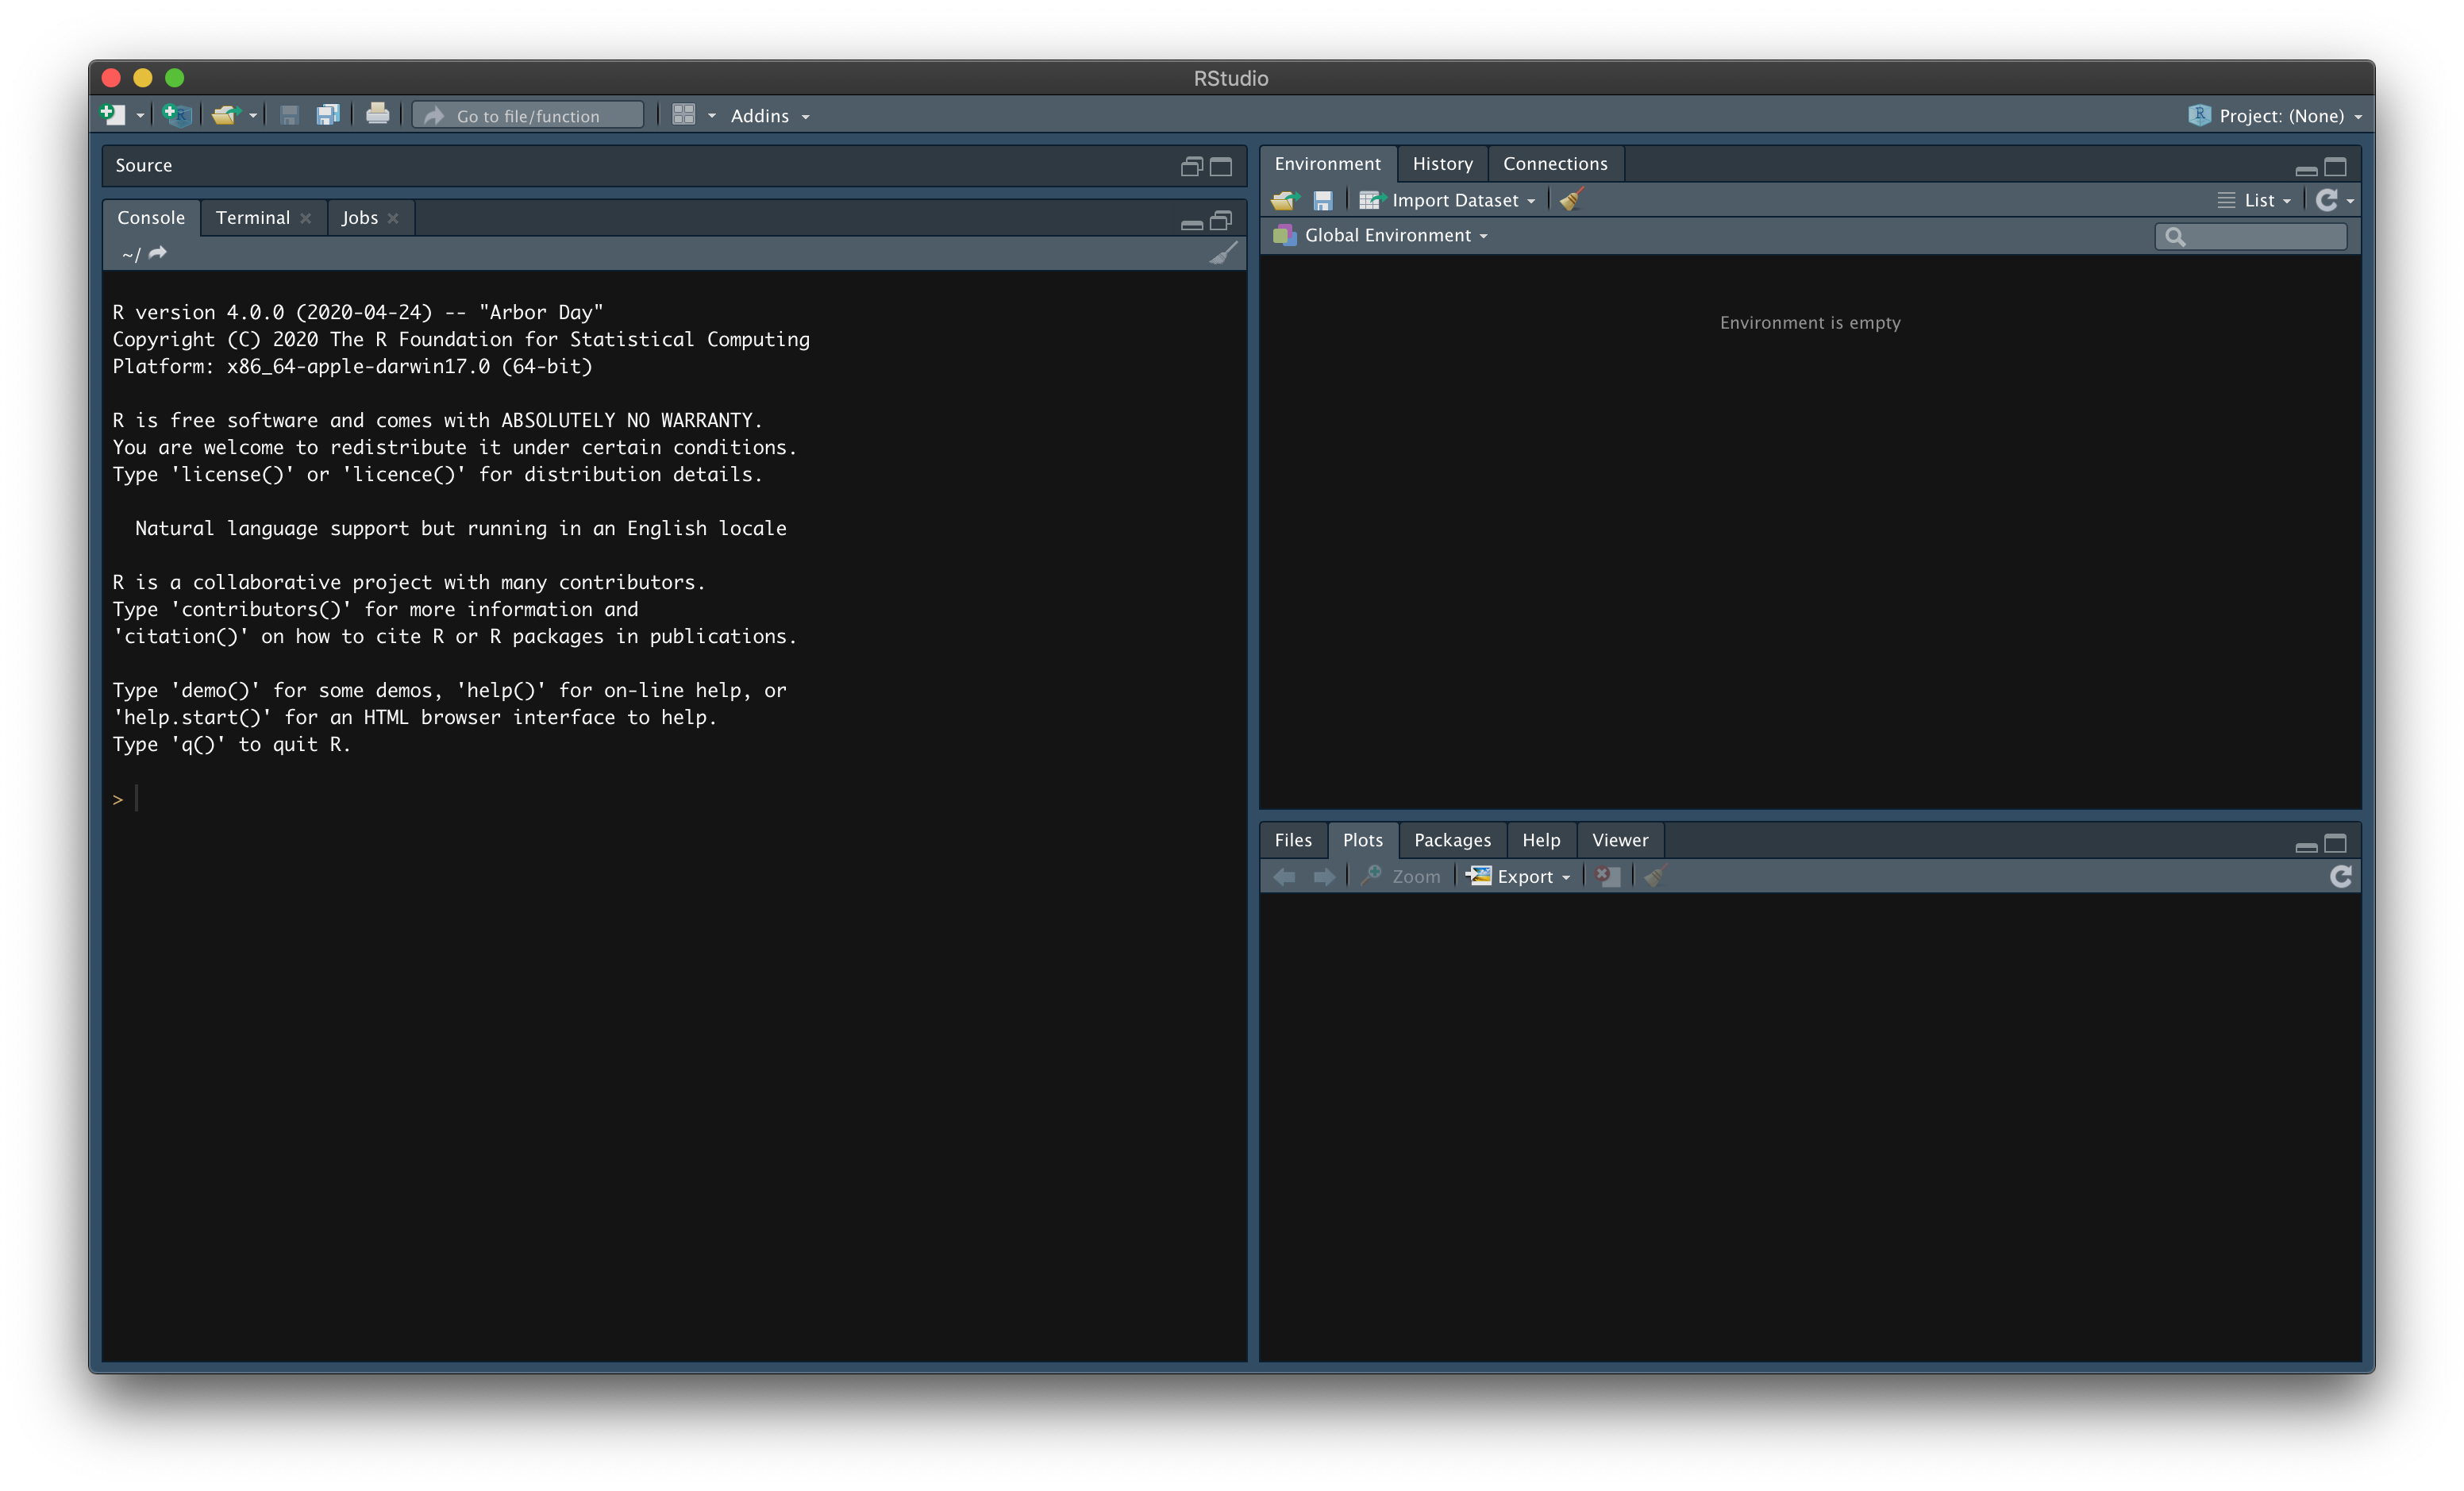
\includegraphics[width=0.8\textwidth]{./images/rstudio.png}
% 		\end{center}
% \end{frame}
% 
% %--- Slide ----------------%
% \begin{frame}{The R Environment}
% \begin{columns}
% 	\begin{column}{0.40\textwidth}
% 	Text editors
% 	\begin{itemize}
% 		\item Inbuilt R Editor
% 		\begin{itemize}
% 			\item File $>$ New Script
% 		\end{itemize}
% 		\item In RStudio
% 		\begin{itemize}
% 			\item Editor panel (top left)
% 		\end{itemize}
% 		\item Copy and record code (especially when successful!)
% 		\item Use for compiling short scripts for particular analysis
% 		%\item Use $#$ for comments
% 	\end{itemize}
% 	\end{column}
% 	\begin{column}{0.59\textwidth}
% 		\begin{center}
% 			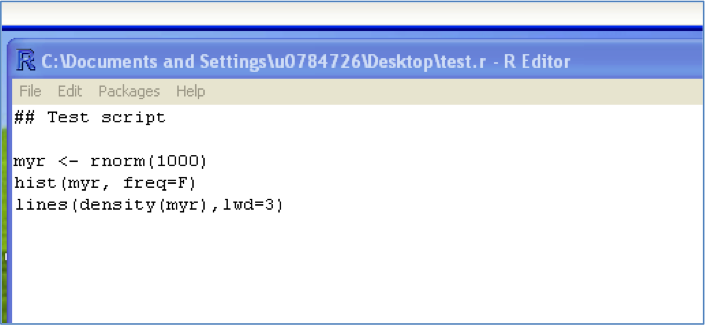
\includegraphics[width=0.94\textwidth]{./images/REditorWin.png}\\
% 			\smallskip
% 			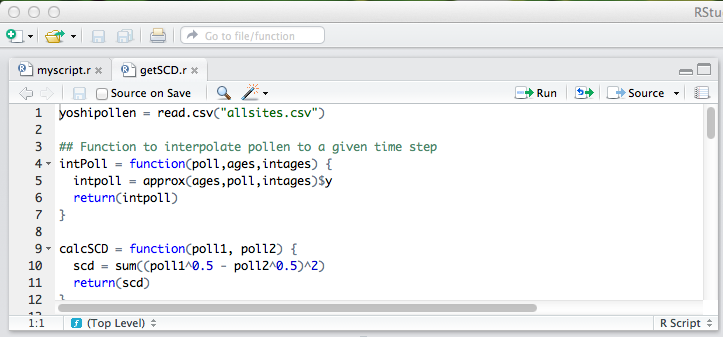
\includegraphics[width=0.94\textwidth]{./images/REditorRStudio.png}
% 		\end{center}
% 	\end{column}
% \end{columns}
% \end{frame}

%--- Slide 20 ----------------%
% \begin{frame}{Next module}
% \begin{itemize}
% 	\item 01: Data import and export, introduction to scripting
% \end{itemize}
% \end{frame}

\end{document}
